\section{Ergebnisse}
\subsection{Laufband}
In \autoref{tab:laufband} sind die eingestellten, ermittelten und berechneten Parameter für die verschiedenen Gangstile des Laufbandexperiments aufgetragen. Der Duty-Faktor beschreibt das Verhältnis von Auftrittsdauer zu Schrittdauer. Er sinkt mit zunehmender Geschwindigkeit ab, bleibt jedoch für alle Geschwindigkeiten über dem kritischen Wert von 0,5. Die Schwungfrequenz steigt nur leicht mit zunehmender Geschwindigkeit, die Schrittfrequenz verdoppelt sich von der geringsten zur höchsten Ganggeschwindigkeit. \\
Aus allen Messreihen (10 Stück) ergibt sich ein durchschnittlicher Wert für die Länge des Bein-Pendels (Abstand Hüfte - Schwerpunkt gesamtes Bein) von 0.37\,m, es ergibt sich hieraus eine Periodendauer von 1,22\,s beziehungsweise eine Frequenz von 0,82\,Hz für den Schwungvorgang. \\
Weiterhin wird ein Vergleich mit dem inversen Pendel-Modell angestrebt. Als Pendellänge wird hierzu die Beinlänge gewählt, welche als 0,94\,m bestimmt wurde. Es ergibt sich dann eine Periodendauer von 1,94\,s. Die Periodendauer der Standphase, also jener Zeit in der die Hüfte um den Standmittelpunkt pendelt, ergibt sich aus der doppelten Dauer einer Standphase. \\

\begin{table}[h!]
	\centering
	\caption[Abgeleitete Größen]{Übersicht der Laufparameter bei den sieben verschiedenen Gehgeschwindigkeiten, welche auf dem Laufband untersucht wurden. Die errechnete Geschwindigkeit wird aus Schrittfrequenz und -weite bestimmt, die gemessene Geschwindigkeit entspricht der Horizontalgeschwindigkeit des Fußes beim Stillstand auf dem Laufband. Die Standperiode wird mit einem Inversen Pendel mit Pendellänge 0,94\,m verglichen. Die subjektive Bewertung geht von 1 (sehr unangenehm) bis 10 (sehr angenehm);}
	\label{tab:laufband}
	\begin{tabular}{L{5.5cm}C{0.9cm}C{0.9cm}C{0.9cm}C{0.9cm}C{0.9cm}C{0.9cm}C{0.9cm}}
		\toprule
		\textbf{Eingestellte Geschw. [kmh]} & 1.00 & 2.00 & 3.00 & 4.00 & 5.00 & 6.00 & 7.00\\
		\midrule 
		\textbf{Duty-Faktor} 		& 0.78 & 0.71 & 0.68 & 0.66 & 0.60 & 0.59 & 0.58 \\
		\textbf{Schwungfrequenz [Hz]} & 1.09 & 1.14 & 1.14 & 1.25 & 1.14 & 1.25 & 1.25 \\
		\textbf{Schrittfrequenz [Hz]} & 0.47 & 0.66 & 0.72 & 0.86 & 0.90 & 1.02 & 1.04 \\
		\textbf{Schrittweite [m] }& 0.37 & 0.50 & 0.69 & 0.75 & 0.85 & 0.88 & 0.97 \\
		\midrule
		\textbf{Errechnete Geschw. [kmh]} & 1.25 & 2.37 & 3.56 & 4.65 & 5.51 & 6.44 & 7.19 \\
		\textbf{Gemessene Geschw. [kmh]} & 0.93 & 1.93 & 3.09 & 4.16 & 5.02 & 6.27 & 7.15 \\
		\midrule
		\textbf{Subj. Bewertung } & 1 & 3 & 6 & 7 & 10 & 6 & 4 \\
		 \textbf{Periode Stand [s]} &  3.32 &  2.15 &  1.89 & 1.53 &  1.33 &  1.15 & 1.12 \\
		\textbf{Abweichung Pendel [\%]}  & +71 & +11 & -3 & -21 & -31 & -41 & -43 \\
%		& 33 & 39 & 39 & 52 & 39 & 52 & 52 \\
		\bottomrule
	\end{tabular}
\end{table}

Im letzten Abschnitt der Tabelle ist der Vergleich der Gangarten mit dem inversen Pendel Modell aufgetragen.\\ 
Es ergibt sich eine minimale Abweichung der Periodendauer von 3\,\%{} für eine Geschwindigkeit für 3\,\kmh. Für langsamere Geschwindigkeiten steigt die Standdauer, bei höheren Geschwindigkeiten sinkt sie. Die als subjektiv am angenehmsten Empfundene Geschwindigkeit ist 5\,\kmh. Am wenigsten angenehm empfunden wurde eine Gehgeschwindigkeit von 1\,\kmh. 

\subsection{Laufstrecke}
Auf der Laufstrecke wurden drei Durchgänge mit vom Probanden als langsam, angenehm und schnell empfundenen Geschwindigkeiten durchgeführt. Eine Übersicht über die verschiedenen Gangstile findet sich in \autoref{tab:laufstrecke}. 
Die Schwungfrequenz steigt mit zunehmender Geschwindigkeit an. Die Schrittfrequenz unterscheidet steigt von 0,93 bei 1,61\,\kmh auf 1,39 bei 8,58\,\kmh um 178\,\% an. 

 \begin{table}[h!]
	\centering
	\caption[Übersicht Laufstrecke]{Parameter der drei gewählten Gehgeschwindigkeiten des Laufstreckenversuchs. Die Geschwindigkeit des Nackens bezieht sich auf die berechnete durchschnittliche Horizontalgeschwindigkeit des Nackenmarkers.}
	\label{tab:laufstrecke}
	\begin{tabular}{L{4.5cm}C{1.5cm}C{2cm}C{2cm}C{2cm}}
		\toprule
		\textbf{Geschw. gefühlt}& langsam & angenehm & schnell \\
		\midrule
		\textbf{Duty-Faktor}	& 0.75 & 0.64 & 0.53 \\
		\textbf{Schwungfrequenz [Hz]} & 0.93 & 1.19 & 1.39 \\
		\textbf{Schrittfrequenz [Hz]} & 0.46 & 0.86 & 1.28 \\
		\textbf{Geschw. Nacken [kmh]}& 1.61 & 4.45 & 8.58 \\
		\bottomrule
		
	\end{tabular}
\end{table}

\subsubsection{Bodenreaktionskräfte}
Die Kräfte, welche von der Waage aufgenommen und in Newton umgerechnet wurden, sind für die drei untersuchten Geschwindigkeiten in \autoref{fig:grf} über den entdimensionierten Schrittzyklus aufgetragen. Die Kräfte wurden nur für die Standphase aufgetragen.\\
Die Bodenreaktionskraft des langsamen Gehens (rote Kurve) beginnt mit einer zunächst kleinen Belastung, welche nach einem kurzen Plateau nahezu linear ansteigt und ein zweites Plateau erreicht und danach wiederum auf 0 absinkt. Das zweite Plateau markiert das Stehen auf einem Bein und dauert etwa 35\,\% des gesamten Schrittzykluses an. Die Bodenreaktionskraft überschreitet zu keinem Zeitpunkt die Gewichtskraft des Probanden.\\

\begin{figure}[h!]
	\centering
	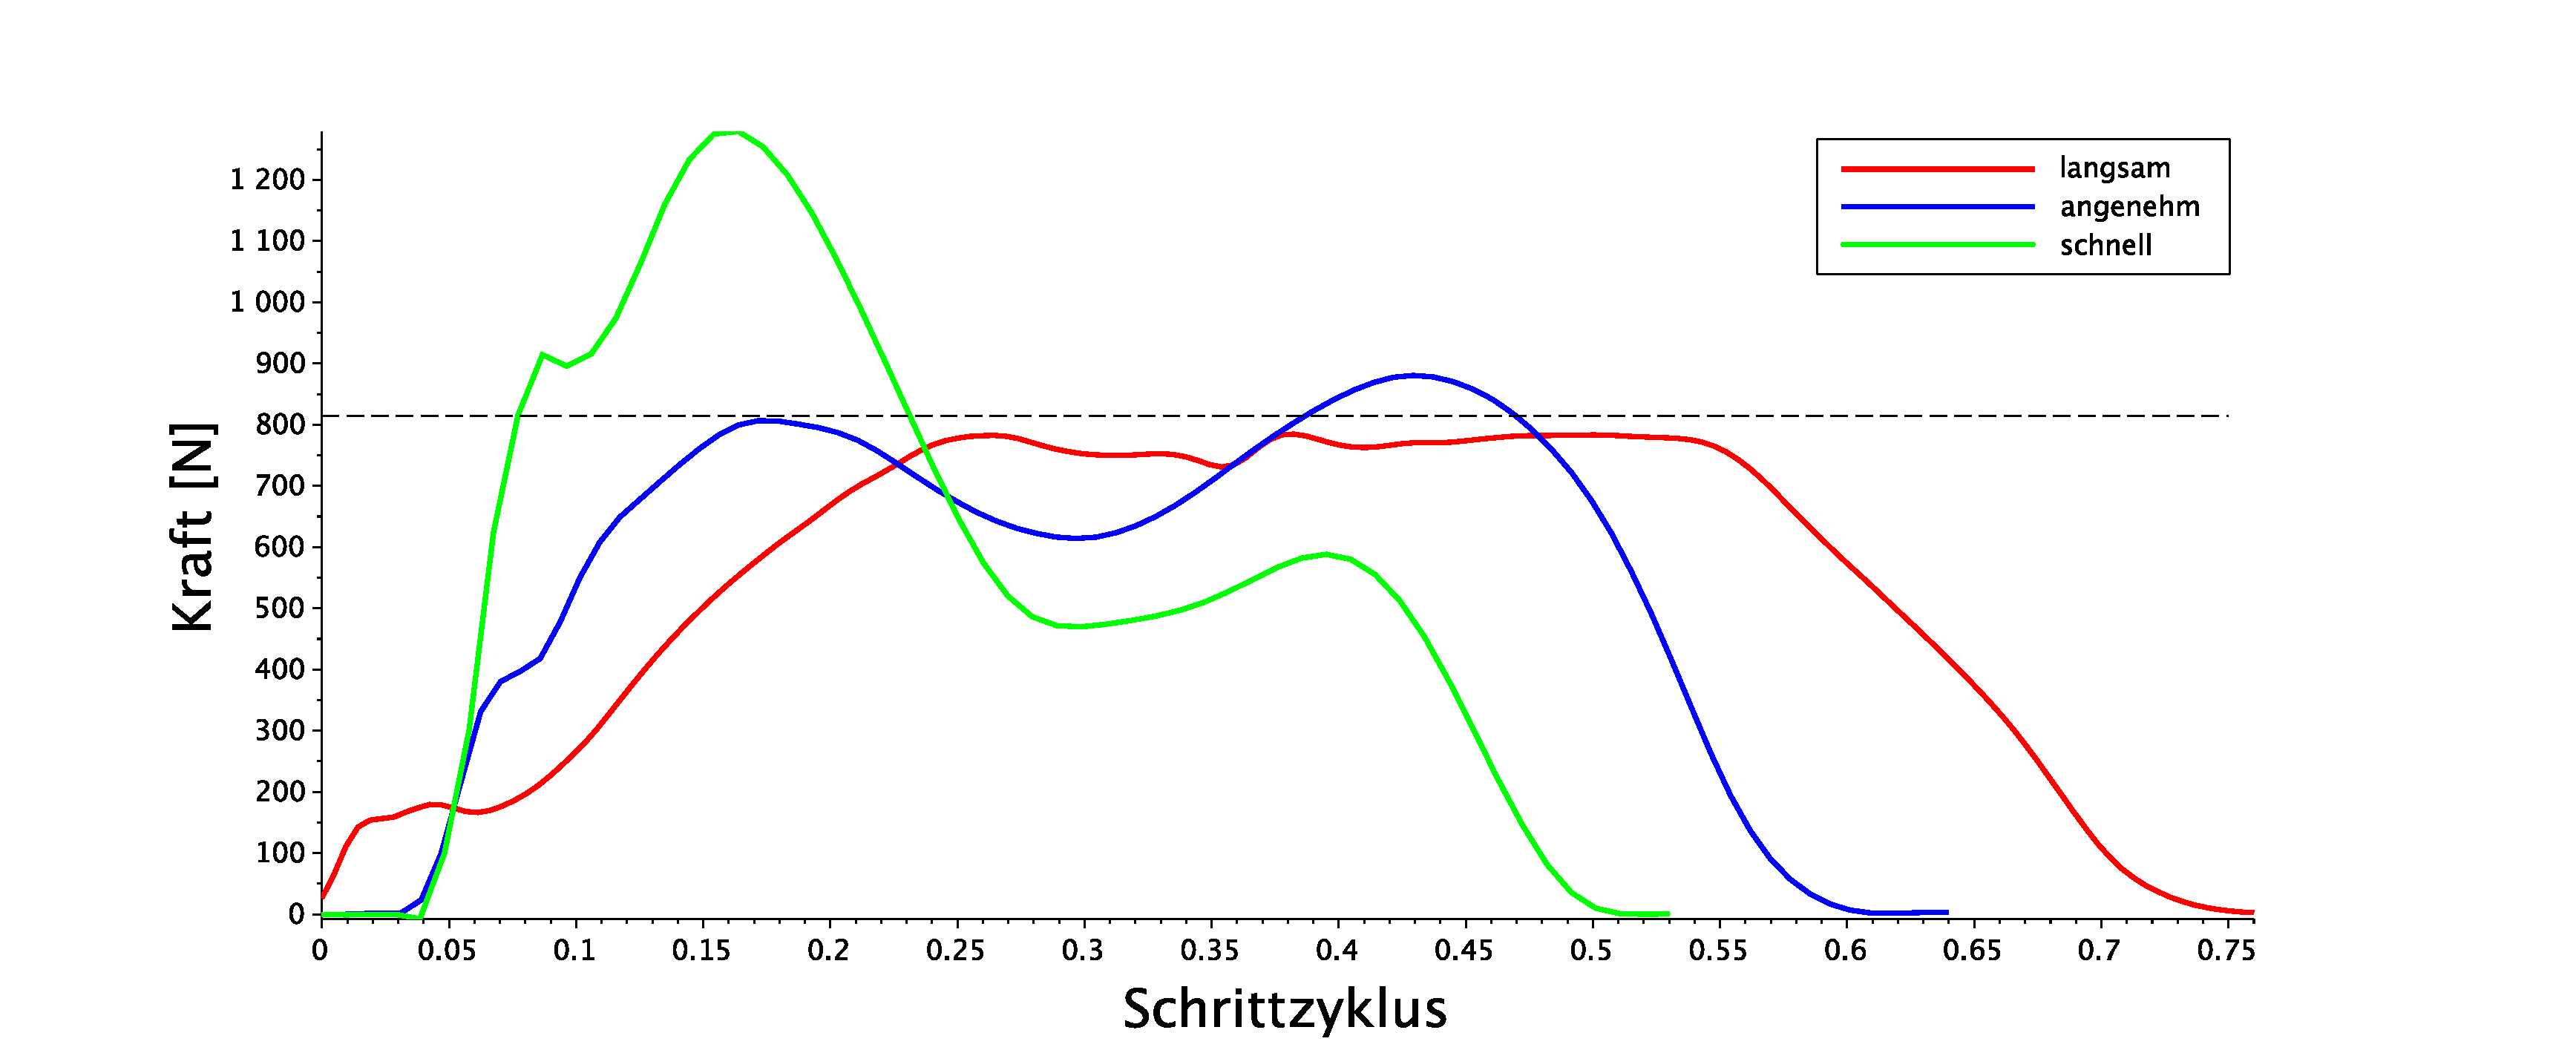
\includegraphics[width=1\linewidth]{bilder/ergebnisse/Forces_df_plusbw.pdf}
	\caption[Bodenreaktionskräfte]{Verlauf der Bodenreaktionskräfte entgegen der Gravitationsrichtung über den entdimensionierten Schrittzyklus. Schwarz gestrichelte Linie: Gewichtskraft des Probanden.}
	\label{fig:grf}
\end{figure}

Das angenehme Gehen (blaue Kurve) ist durch drei charakteristische Höcker gekennzeichnet. Direkt nach Beginn der Belastung zeigt sich ein kleinerer Knick, woraufhin die Belastung weiter ansteigt und den Wert der Gewichtskraft erreicht. Die Belastung sinkt daraufhin auf ein lokales Minimum von 609\,N ab, was 75\,\% der Gewichtskraft entspricht. Im weiteren Verlauf steigt die Bodenreaktionskraft erneut an auf 880\,N beziehungsweise 108\,\% der Gewichtskraft. \\
Die Kräfte des schnellen Gehens sind in grün eingezeichnet. Sie steigen zunächst stark an und weisen einen ersten Knick bei 905\,N auf. Das im weiteren Verlauf erreichte Maximum von 1275\,N (156\,\% Gewichtskraft) wird nach etwa einem fünftel der Standdauer erreicht. Die Bodenreaktionskraft sinkt daraufhin ab und erreicht ein weiteres Plateau und ein lokales Maximum von 582\,N, bevor sie auf null absinkt.\\

\subsubsection{Inverse Dynamik}
Neben den in \autoref{fig:grf} aufgetragenen vertikalen Kräften wurden zudem die Kräfte in Laufrichtung und quer zur Laufrichtung aufgenommen. Über die inverse Dynamik lassen sich so die Kräfte in den Gelenken berechnen.
In \autoref{fig:knee_forces} sind für das Knie die Kräfte in Laufrichtung (Fx), entgegen der Gravitation (Fy) und das Moment um die Achse senkrecht zur Bildebene für die angenehme Geschwindigkeit aufgetragen. Die Kräfte sind hier nur für die Dauer der Standphase eingezeichnet. Der Verlauf von Fy (blau) ist von zwei Höckern gezeichnet, weist im Vergleich zu den Bodenreaktionskräften jedoch keinen anfänglichen Knick auf. Die in rot eingetragenen Kräfte in Laufrichtung (Fx), sind zunächst negativ, nach etwas mehr als der Hälfte der Belastungsdauer wechseln sie ins positive mit einem maximalen Wert von 112\,N. 
\textbf{DAS DUMME MOMENT MACHT NICHT WAS ES SOLL?}
\begin{figure}[h!]
	\centering
	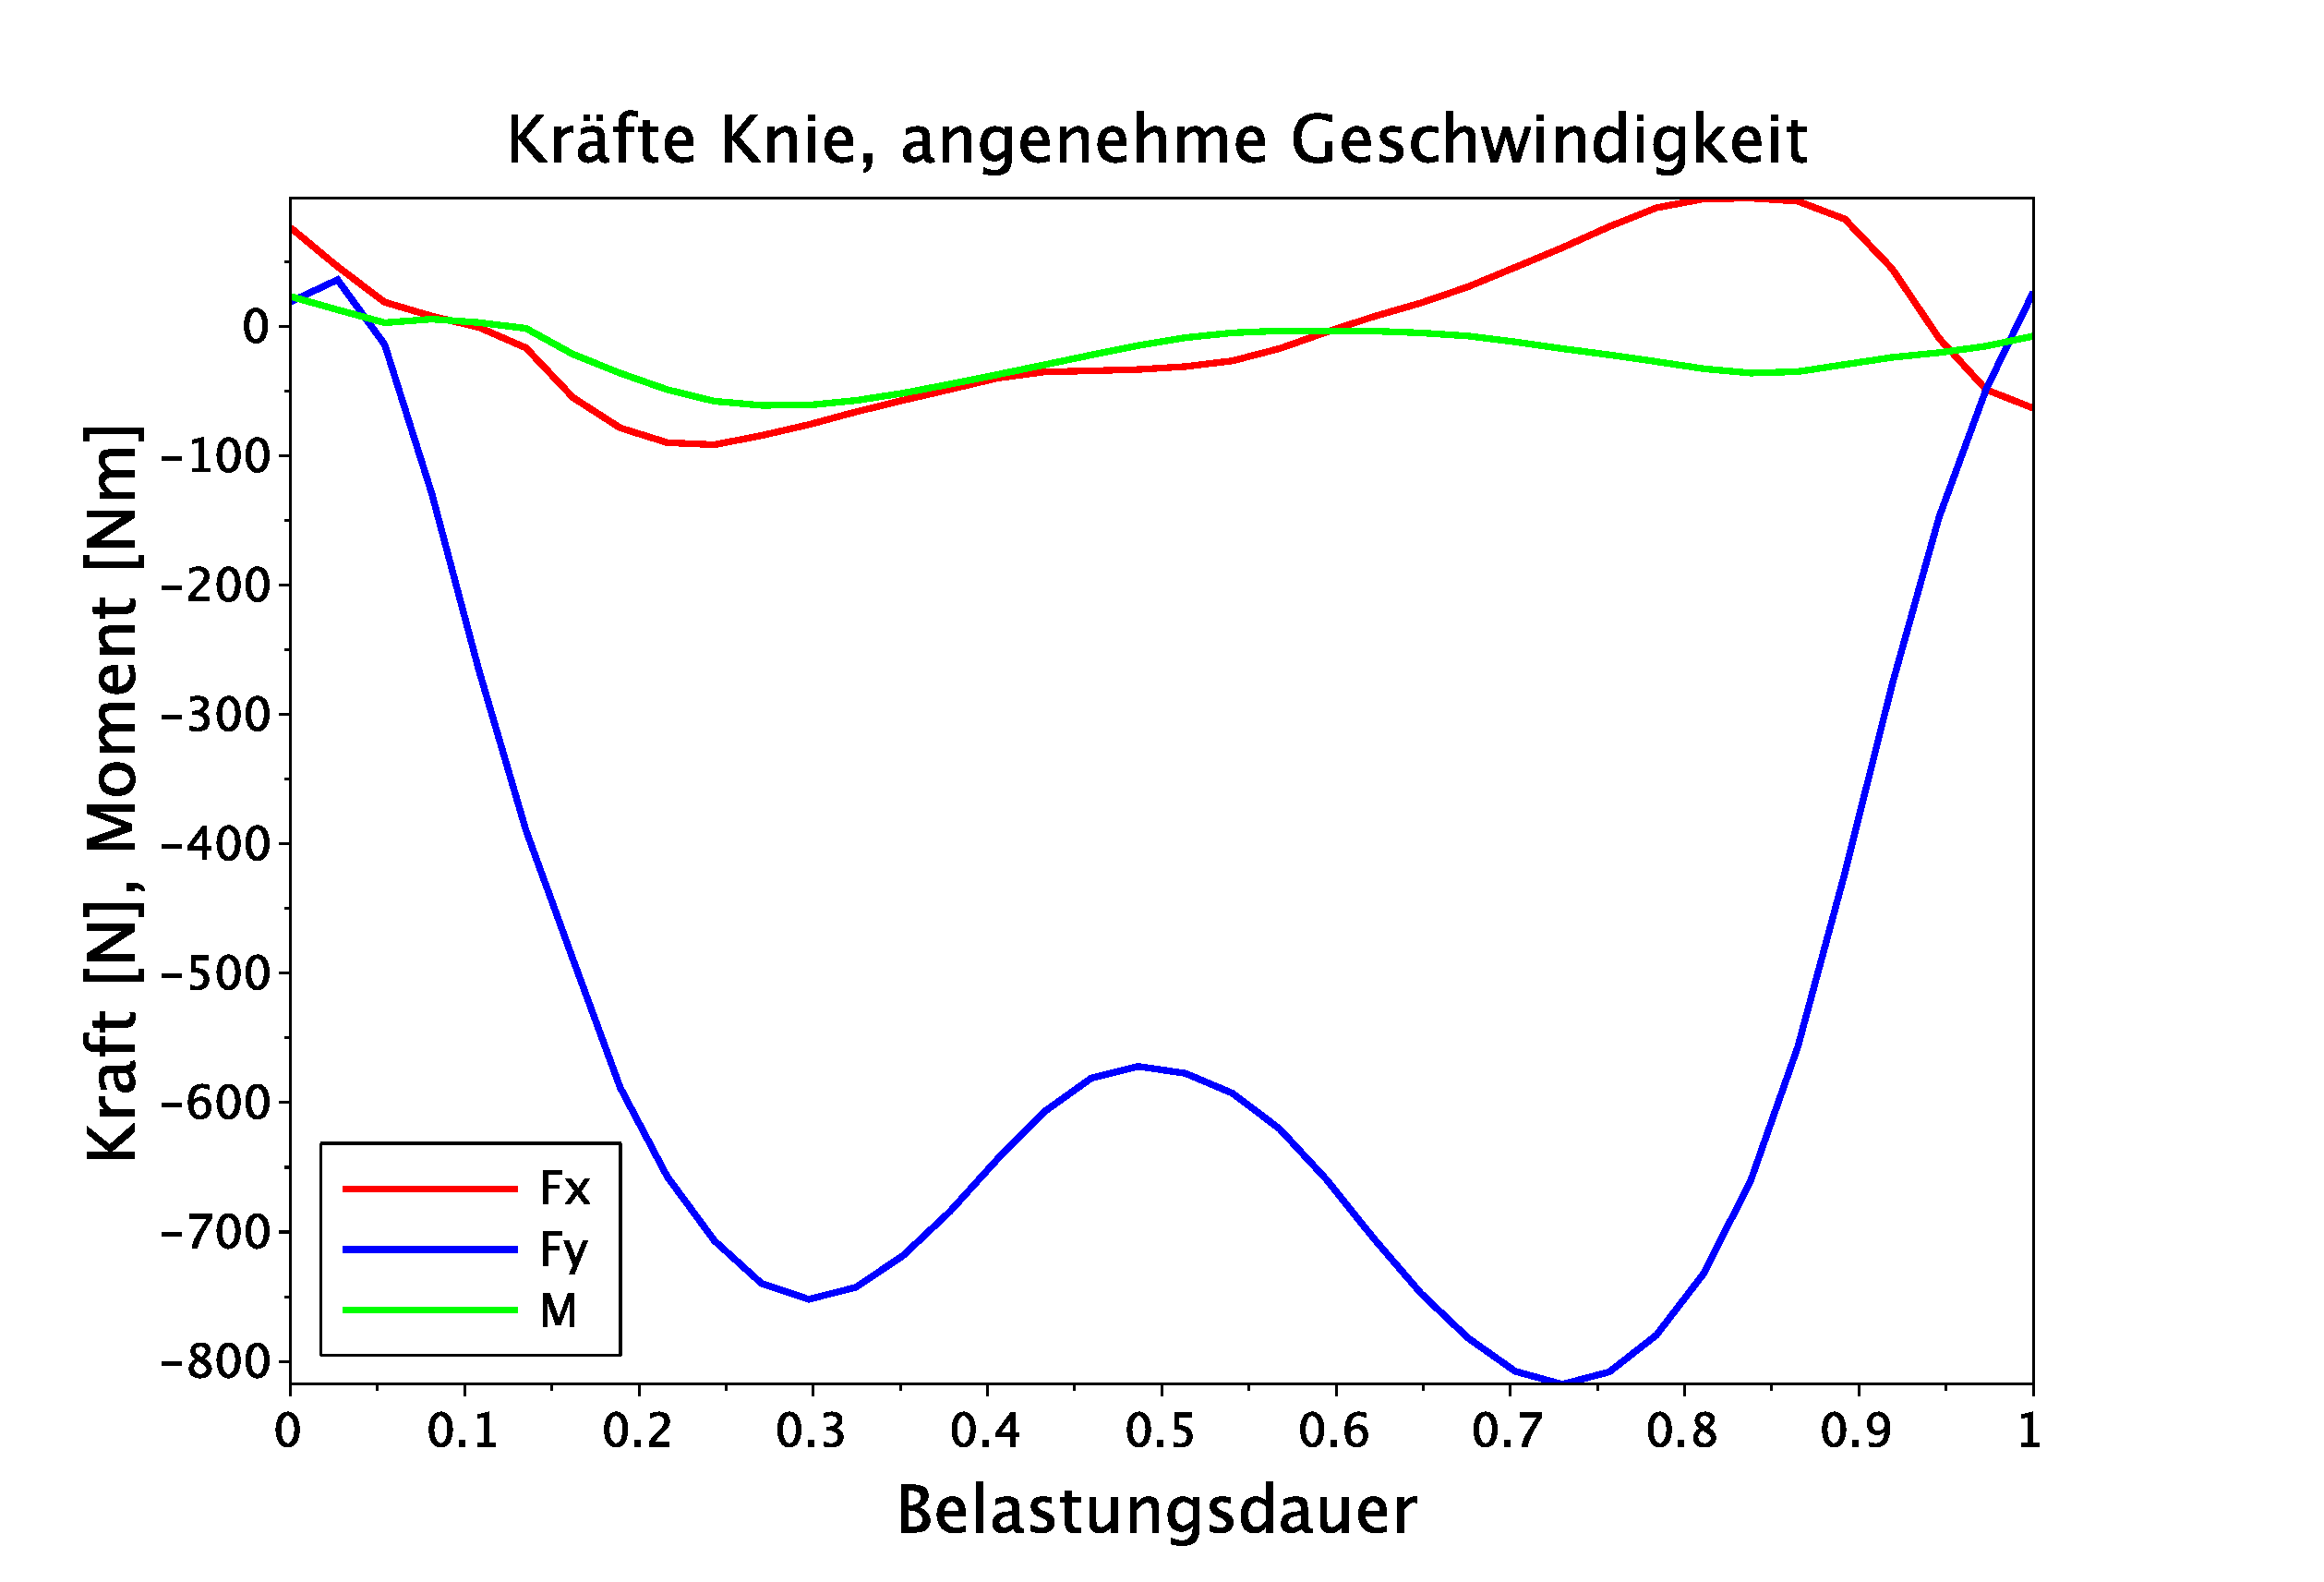
\includegraphics[width=0.7\linewidth]{bilder/ergebnisse/forces_knee.pdf}
	\caption[Bodenreaktionskräfte]{Verlauf von $F_x$, $F_y$ und $M$ während der Standphase.}
	\label{fig:knee_forces}
\end{figure}

Für einen Vergleich der bei verschiedenen Geschwindigkeiten wirkenden Kräfte sind in \autoref{fig:ankle_fx} die Laufrichtung wirkenden Kräfte (Fx) geplottet. Für eine bessere Vergleichbarkeit wurden alle Geschwindigkeiten auf eine gemeinsame x-Achse, der entdimensionierten Belastungsdauer, aufgetragen. Allen Kurven ist gemein, dass sie im positiven starten, ins negative abfallen und nach etwa der halbe Belastungsdauer ins positive Wechseln. Die Kraftverläufe sind dabei annähernd punktsymmetrisch zum Nulldurchgang. Die beim langsamen Gehen auftretenden Kräfte sind kleiner als die der höheren Geschwindigkeiten. Die größte negative Kraft beträgt -32\,N, die größte positive Kraft beträgt 59\,N. \\
Das angenehme Gehen (blau) weist einen ähnlichen Verlauf, mit größeren Extremwerten von -109 und 124\,N. Die Kräfte, welche beim schnellen Gehen auftreten sind noch größer, mit -163 und 132\,N. Im Gegensatz zu den langsameren Geschwindigkeiten ist hier der Betrag des negativen Extremwertes größer als der des später auftretenden positiven Extremwertes.\\
\begin{figure}[h!]
	\centering
	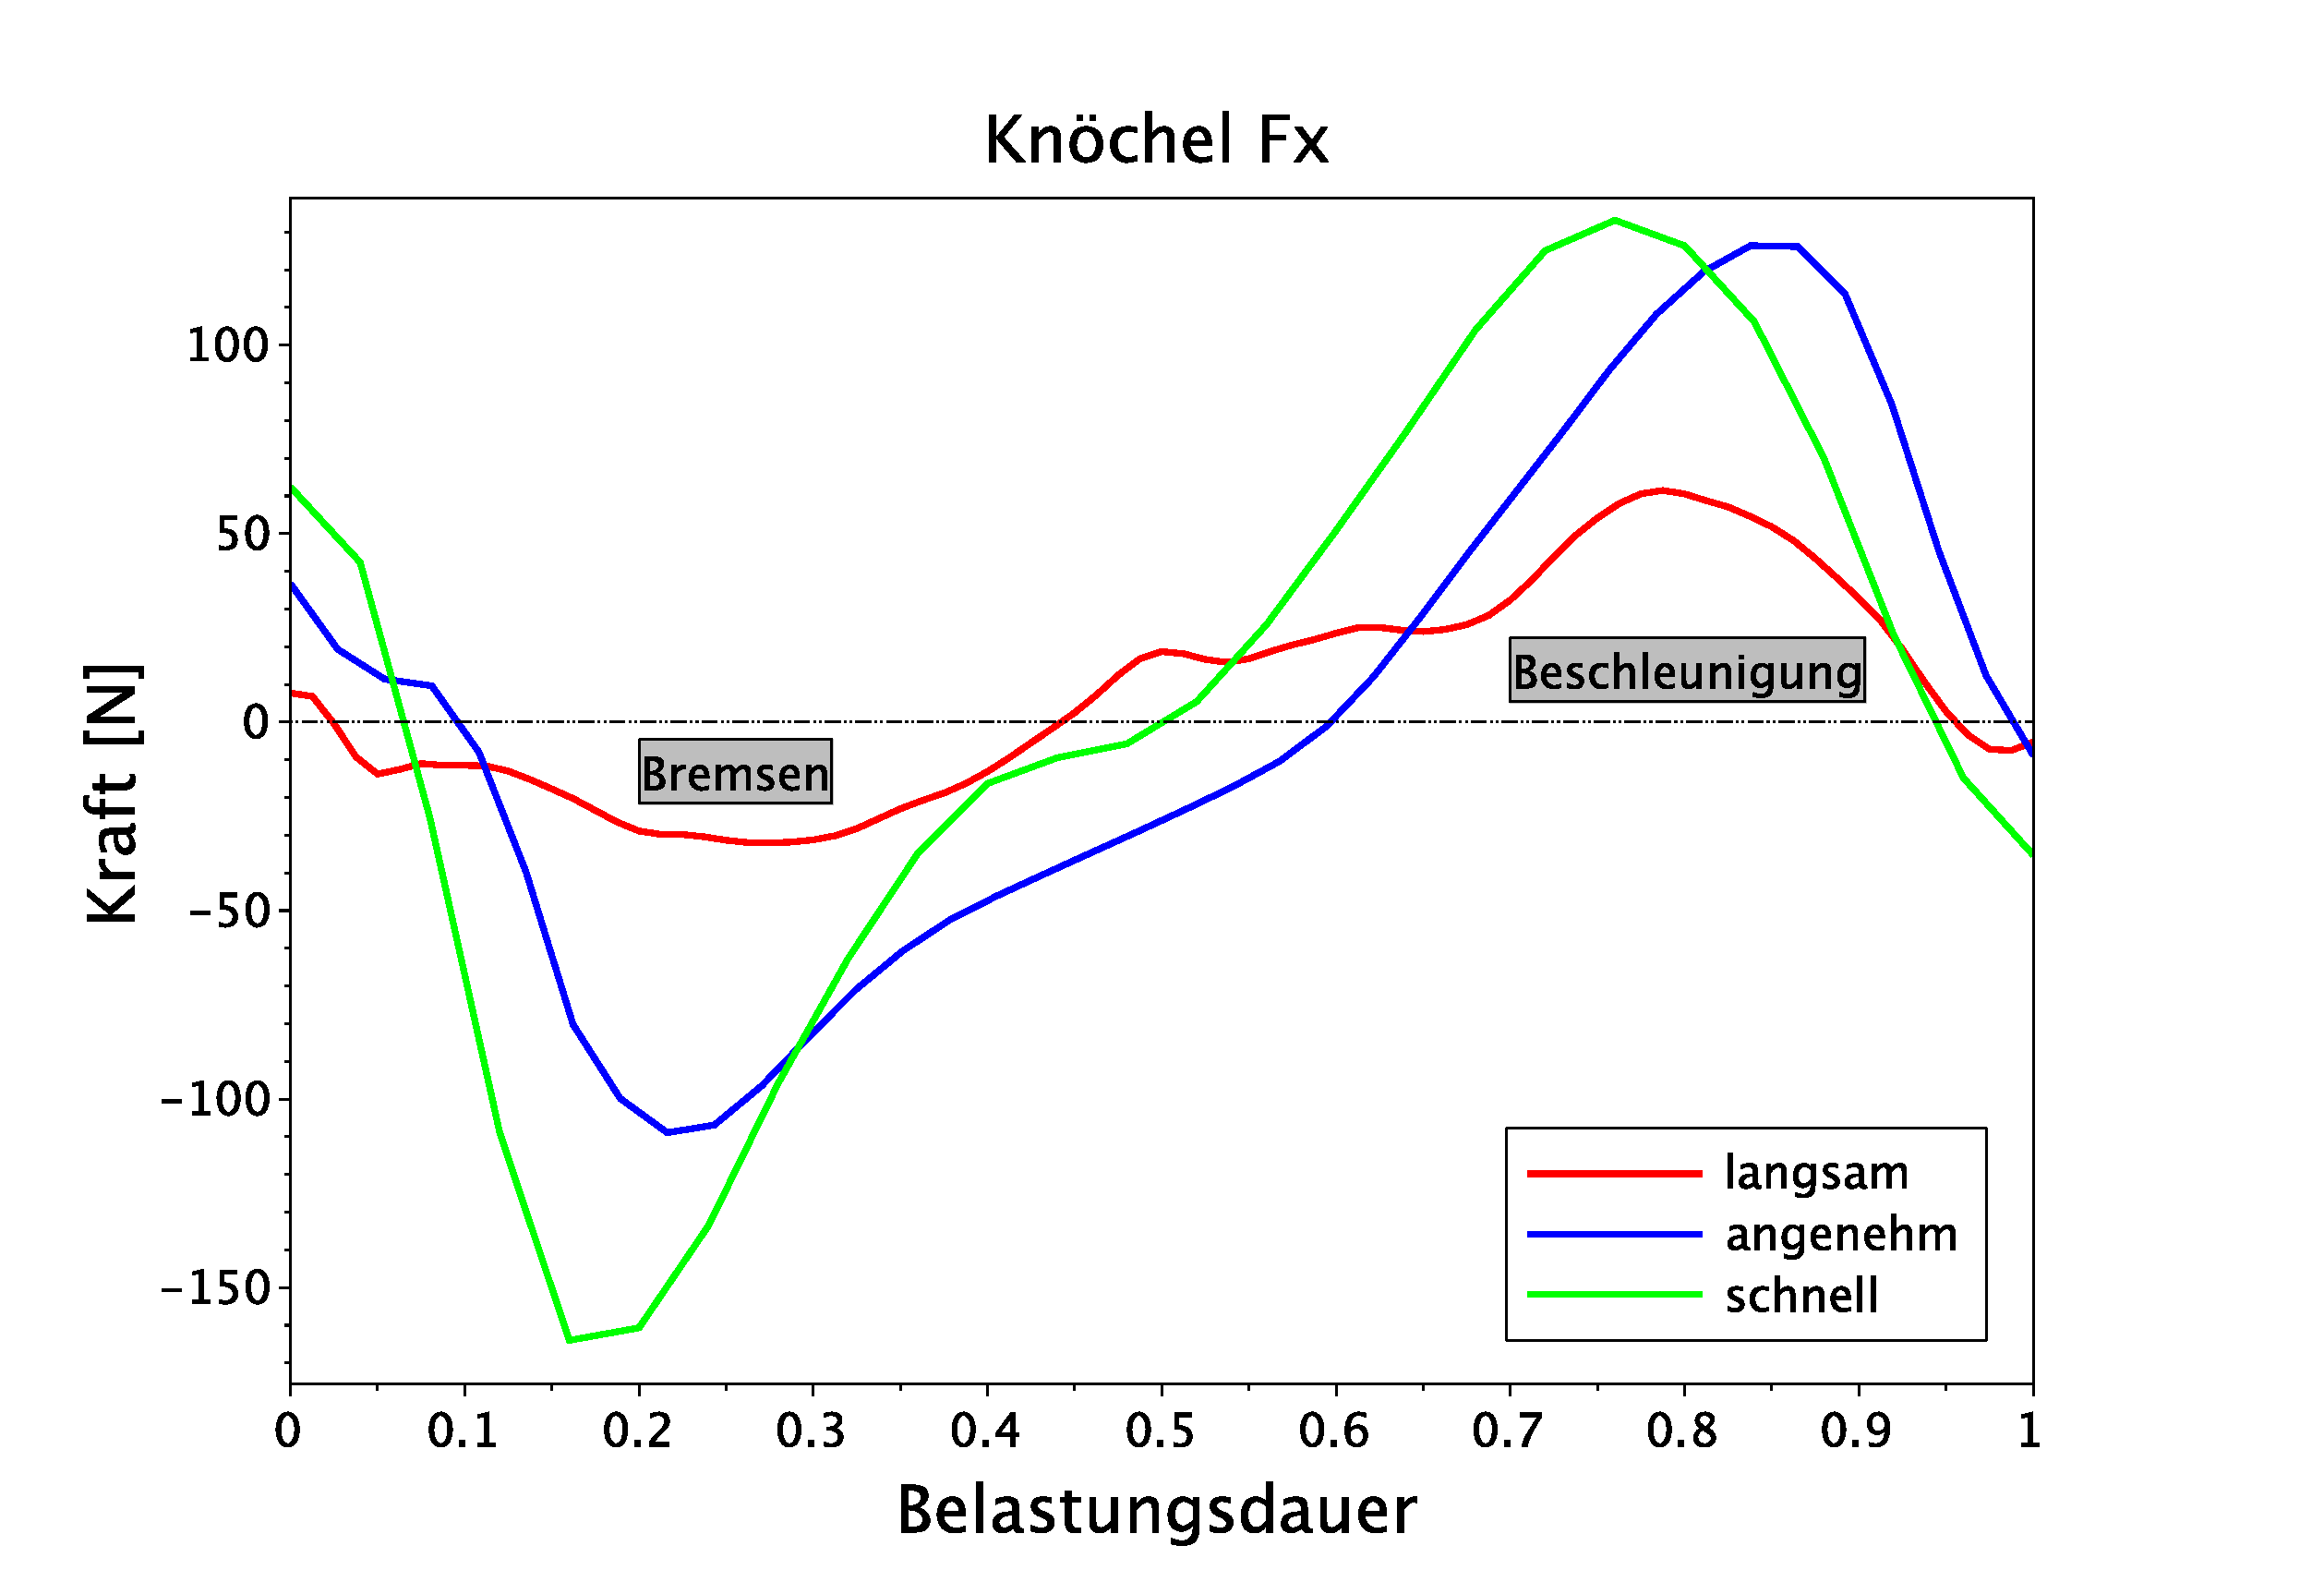
\includegraphics[width=0.7\linewidth]{bilder/ergebnisse/ankle_fx_plot.pdf}
	\caption[Bodenreaktionskräfte]{Verlauf von $F_x$ im Knöchel während der Standphase. Negative Kräfte treten zu Beginn der Standphase auf, Ab der mittleren Standphase treten positive Kräfte auf.}
	\label{fig:ankle_fx}
\end{figure}

Aus sportmedizinischer Sicht interessant sind die bei der Lokomotion auftretenden Momente im verletzungsanfälligen Knie, welche in \autoref{fig:knee_m} eingezeichnet sind. 

\begin{figure}[h!]
	\centering
	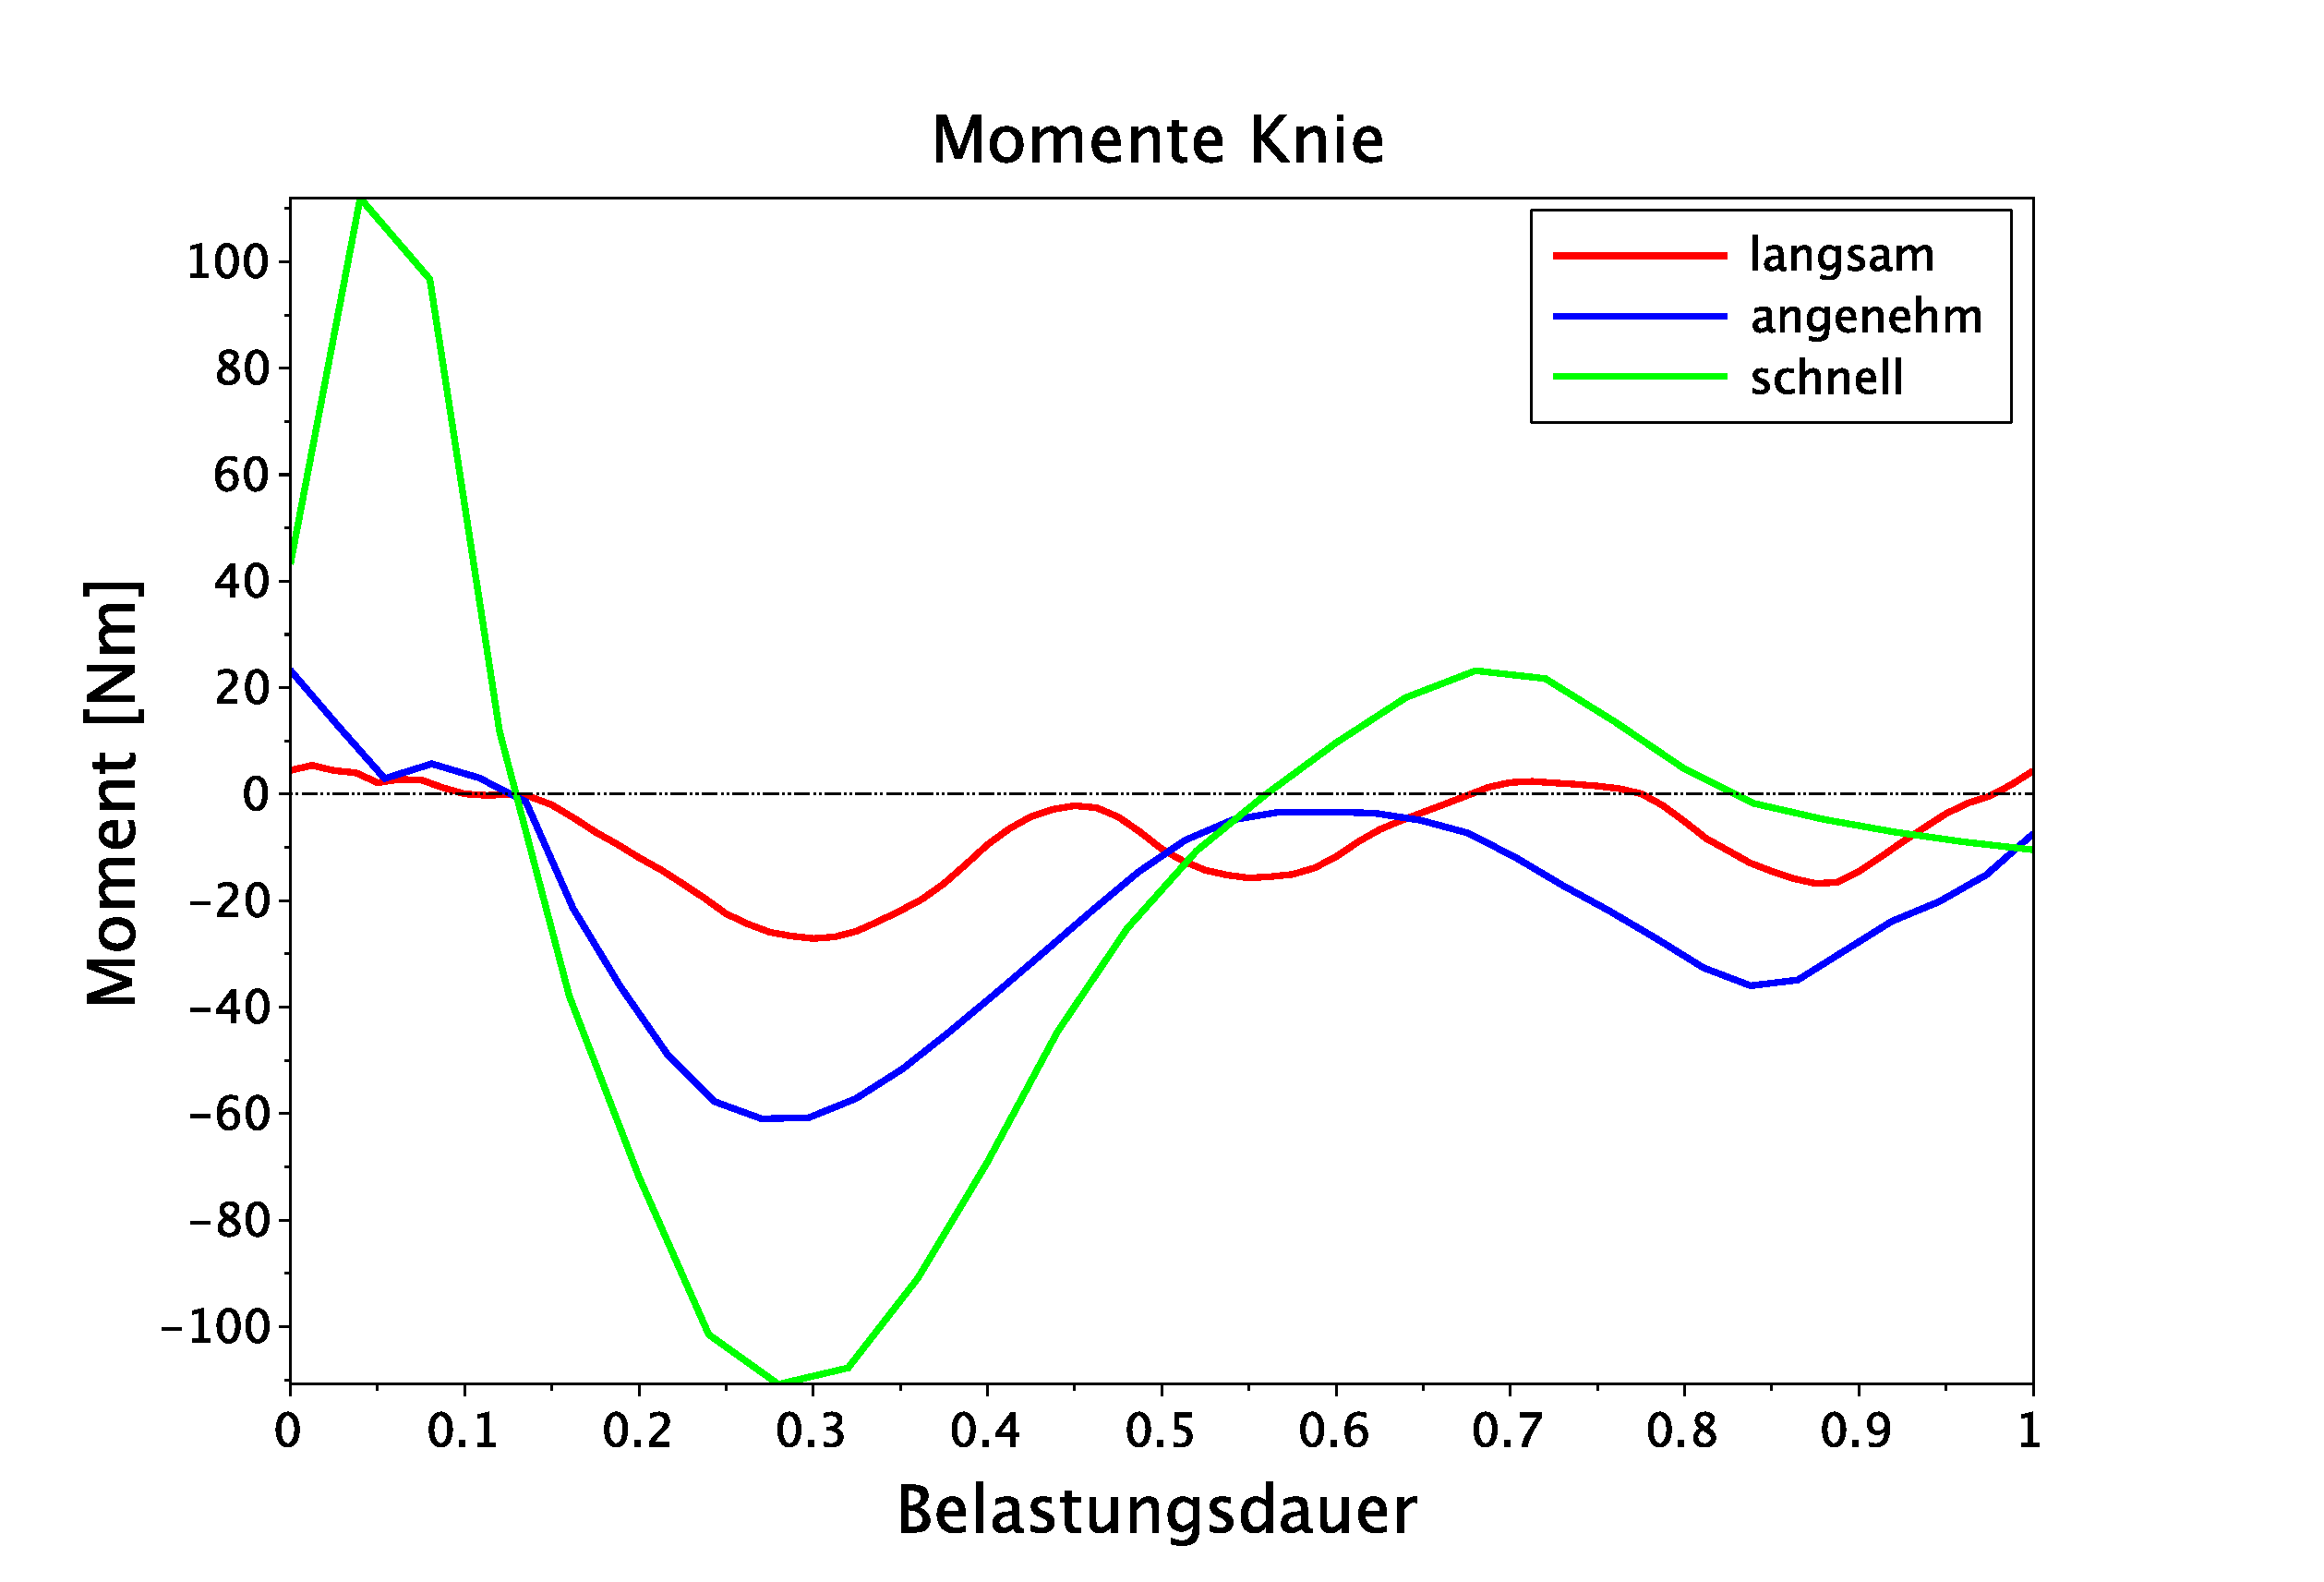
\includegraphics[width=0.7\linewidth]{bilder/ergebnisse/momente_knie.pdf}
	\caption[Bodenreaktionskräfte]{Verlauf von $F_x$, $F_y$ und $M$ während der Standphase.}
	\label{fig:knee_m}
\end{figure}


\subsection{Vergleich Laufband und Laufstrecke}
\textbf{Vergleich Laufstrecke und Laufband}\\
Mithilfe von Winkelmessungen des Oberkörpers, Arme und Beine können die beiden Gangarten verglichen und analysiert werden\\
Die Armbewegungen, welcher in \autoref{fig:vergleich_hand} zu sehen ist, lassen einen Vergleich zwischen den beiden Versuchsaufbauten, sowie unter den Geschwindigkeiten zu. In blautönen eingetragen sind dabei die Versuche auf dem Laufband, in rottönen die auf der Laufstrecke. \\
Die x- und y-Achse geben den horizontalen, bzw. vertikalen Abstand zum Nacken wieder. Je weiter links unten eine Trajektorie sich befindet, umso ausgestreckter ist der Arm.\\
Auf dem Laufband ist die Amplitude des Handgelenkes bei der niedrigsten eingezeichneten Geschwindigkeit von 2\,\kmh (cyan) 0,52\,m, die bei 4\,\kmh beträgt 0,57\,m und die der höchsten Geschwindigkeit (7\,\kmh, dunkelblau) 0,62\,m. 

0,35, 0,10, 0,73


\begin{figure}[h!]
	\centering
	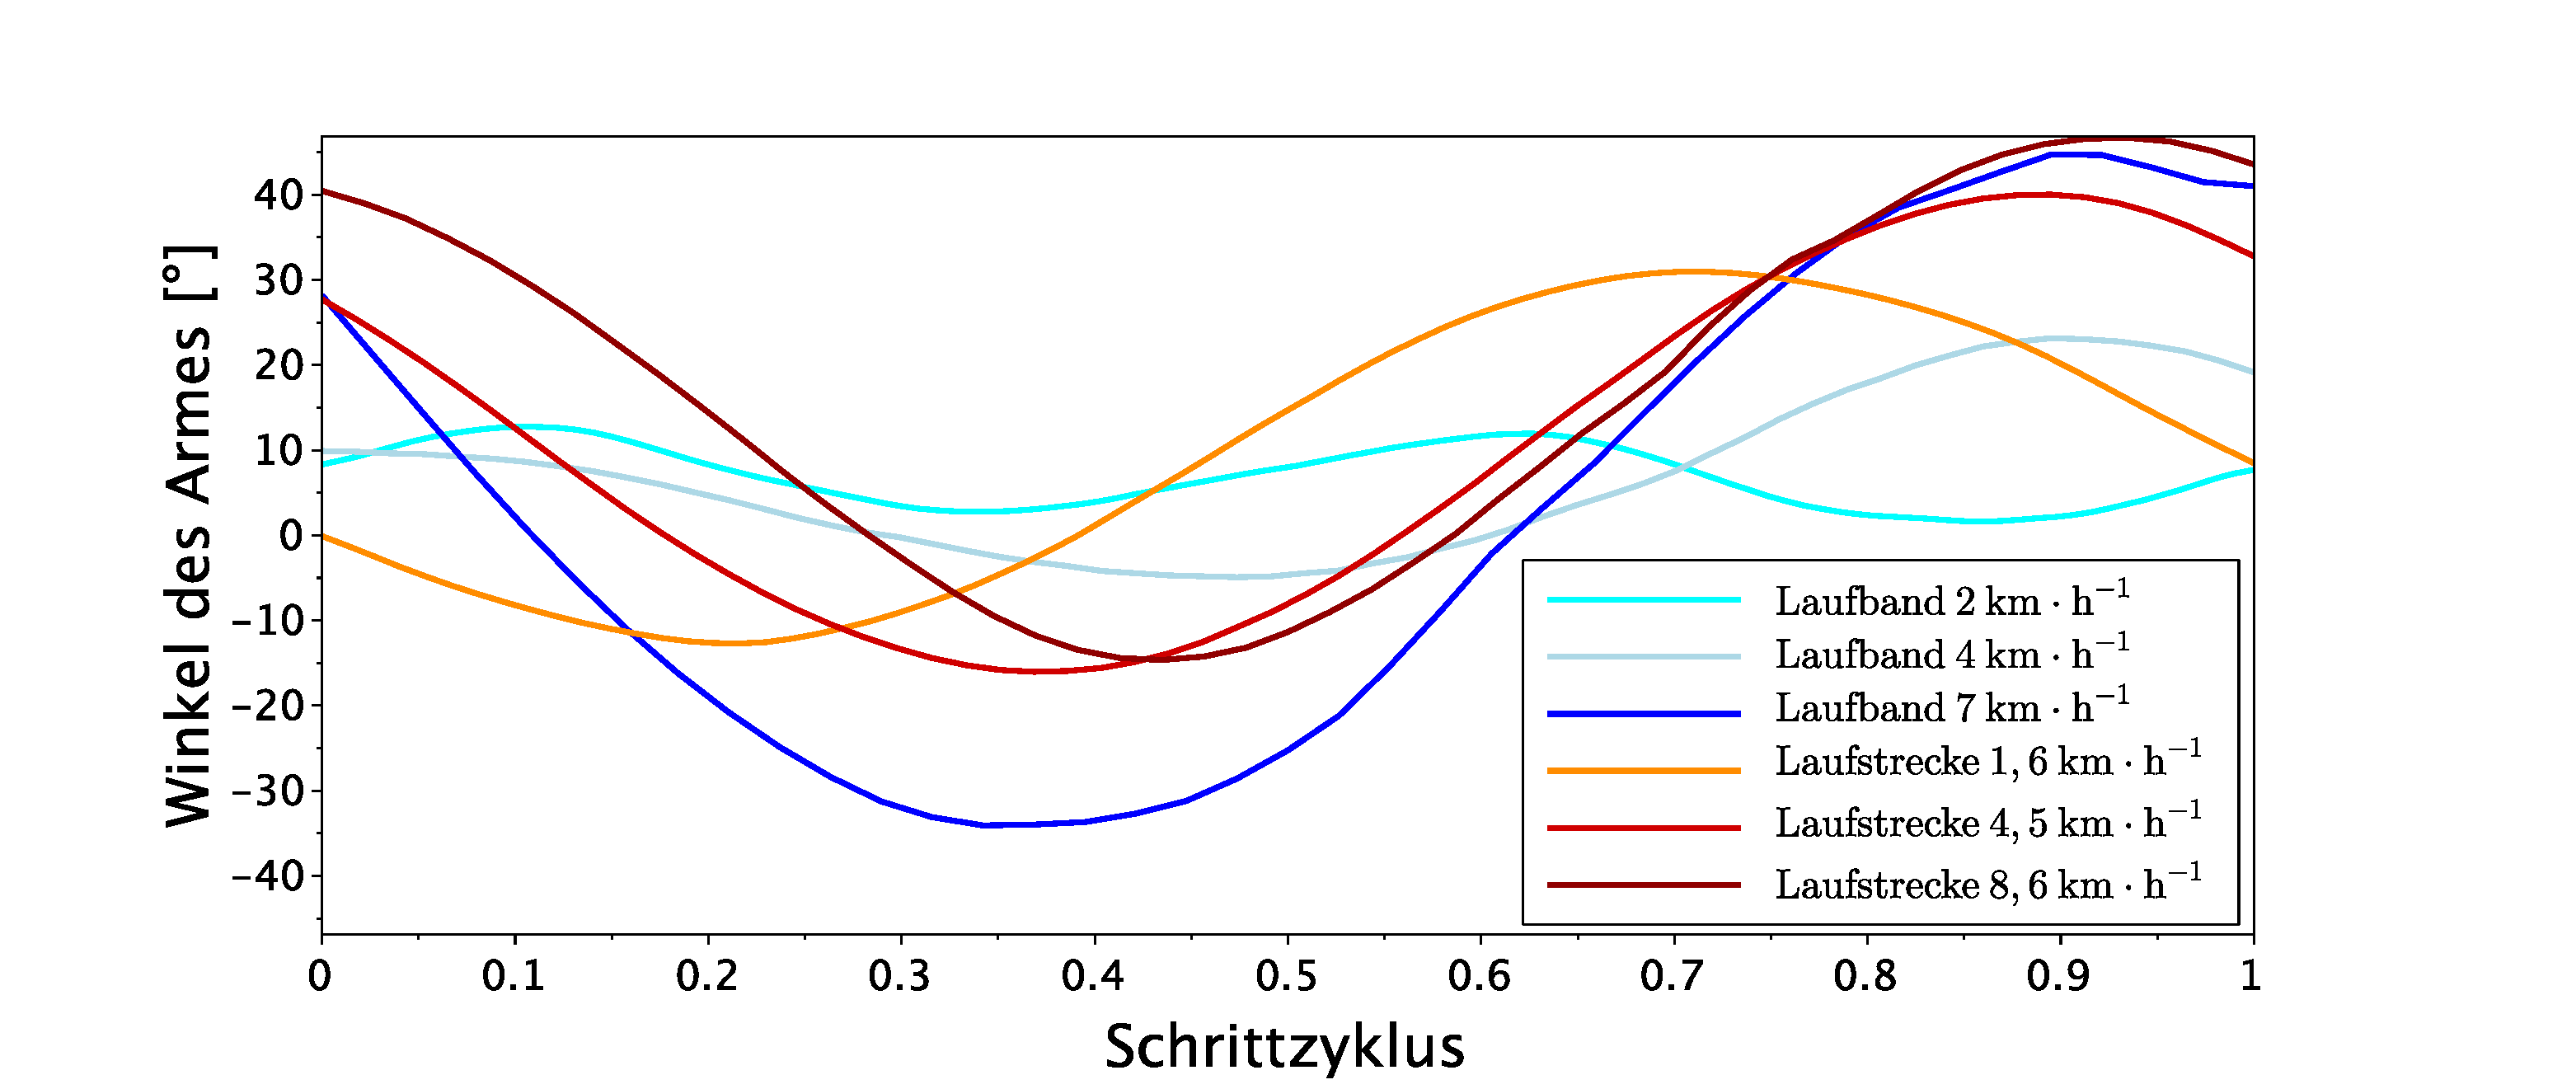
\includegraphics[width=1\linewidth]{bilder/ergebnisse/armschwung_winkel.pdf}
	\caption[Handtrajektorie]{Bewegung des Handgelenks, relativ zum Nacken. Negative x-Werte entsprechen einem Vorschwung, positive Werte einem Zurückschwingen. Auf der Laufstrecke ändert sich die relative Haltung des Handgelenks nach einem Schrittzyklus.}
	\label{fig:vergleich_hand}
\end{figure}

Ein weiterer Vergleich zwischen den Experimenten ist in \autoref{fig:vergleich_oberkörper} zu sehen. Eingetragen sind die relativen Neigungswinkel der Strecke Hüfte - Nacken. Ein Winkel von null Grad entspricht dem aufrechten Stehen, wenn der Nackenmarker senkrecht über dem Hüftmarker steht. Bei positiven Winkeln ist der Nackenmarker in Laufrichtung weiter vorne, bei negativen weiter hinten. Die Werte des Laufbandversuchs sind in Blautönen eingefärbt (cyan, graublau, dunkelblau), die Laufstreckenergebnisse in Rottönen (orange, rot, rotbraun). Allen Kurven gemein ist, dass während des Schrittzykluses der Winkel abfällt und daraufhin wieder ansteigt. Das Minimimum von vier Kurven liegt jeweils bei etwa 50\,\% der Schrittdauer. Einen klaren Unterschied zeigen die jeweils langsamsten Gehgeschwindigkeiten (cyan und orange), mit einer geringen Amplitude von 4,74 und 4,41 Grad und einem periodischen Wanken. Die größten Amplituden finden sich bei den höchsten Geschwindigkeiten mit 12,74 und 10,24 Grad für 7 (dunkelblau), beziehungsweise 8,6\,\kmh.

\begin{figure}[h!]
	\centering
%	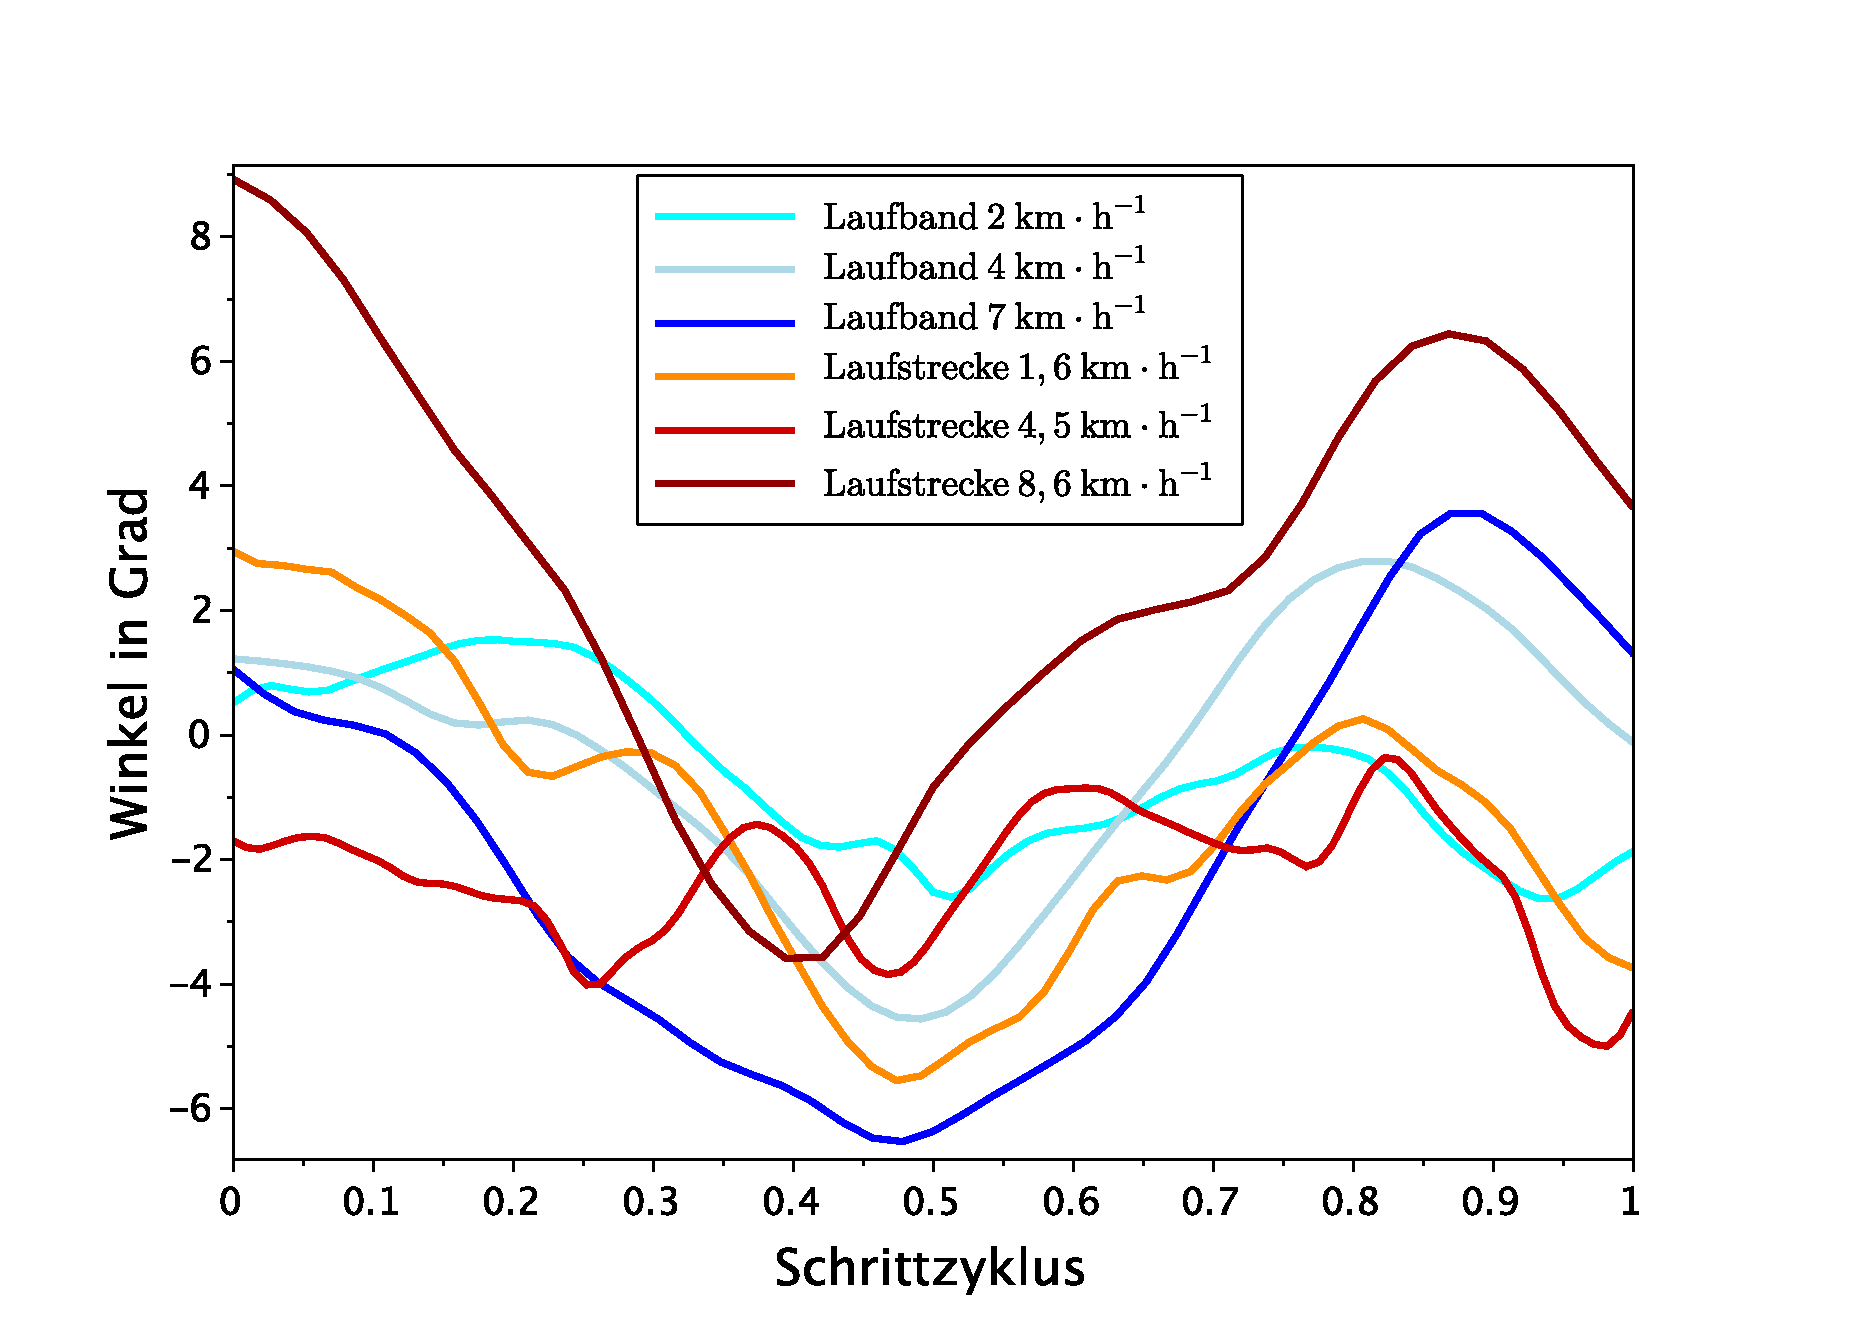
\includegraphics[width=0.7\linewidth]{bilder/ergebnisse/winkel_vergleich.pdf}
	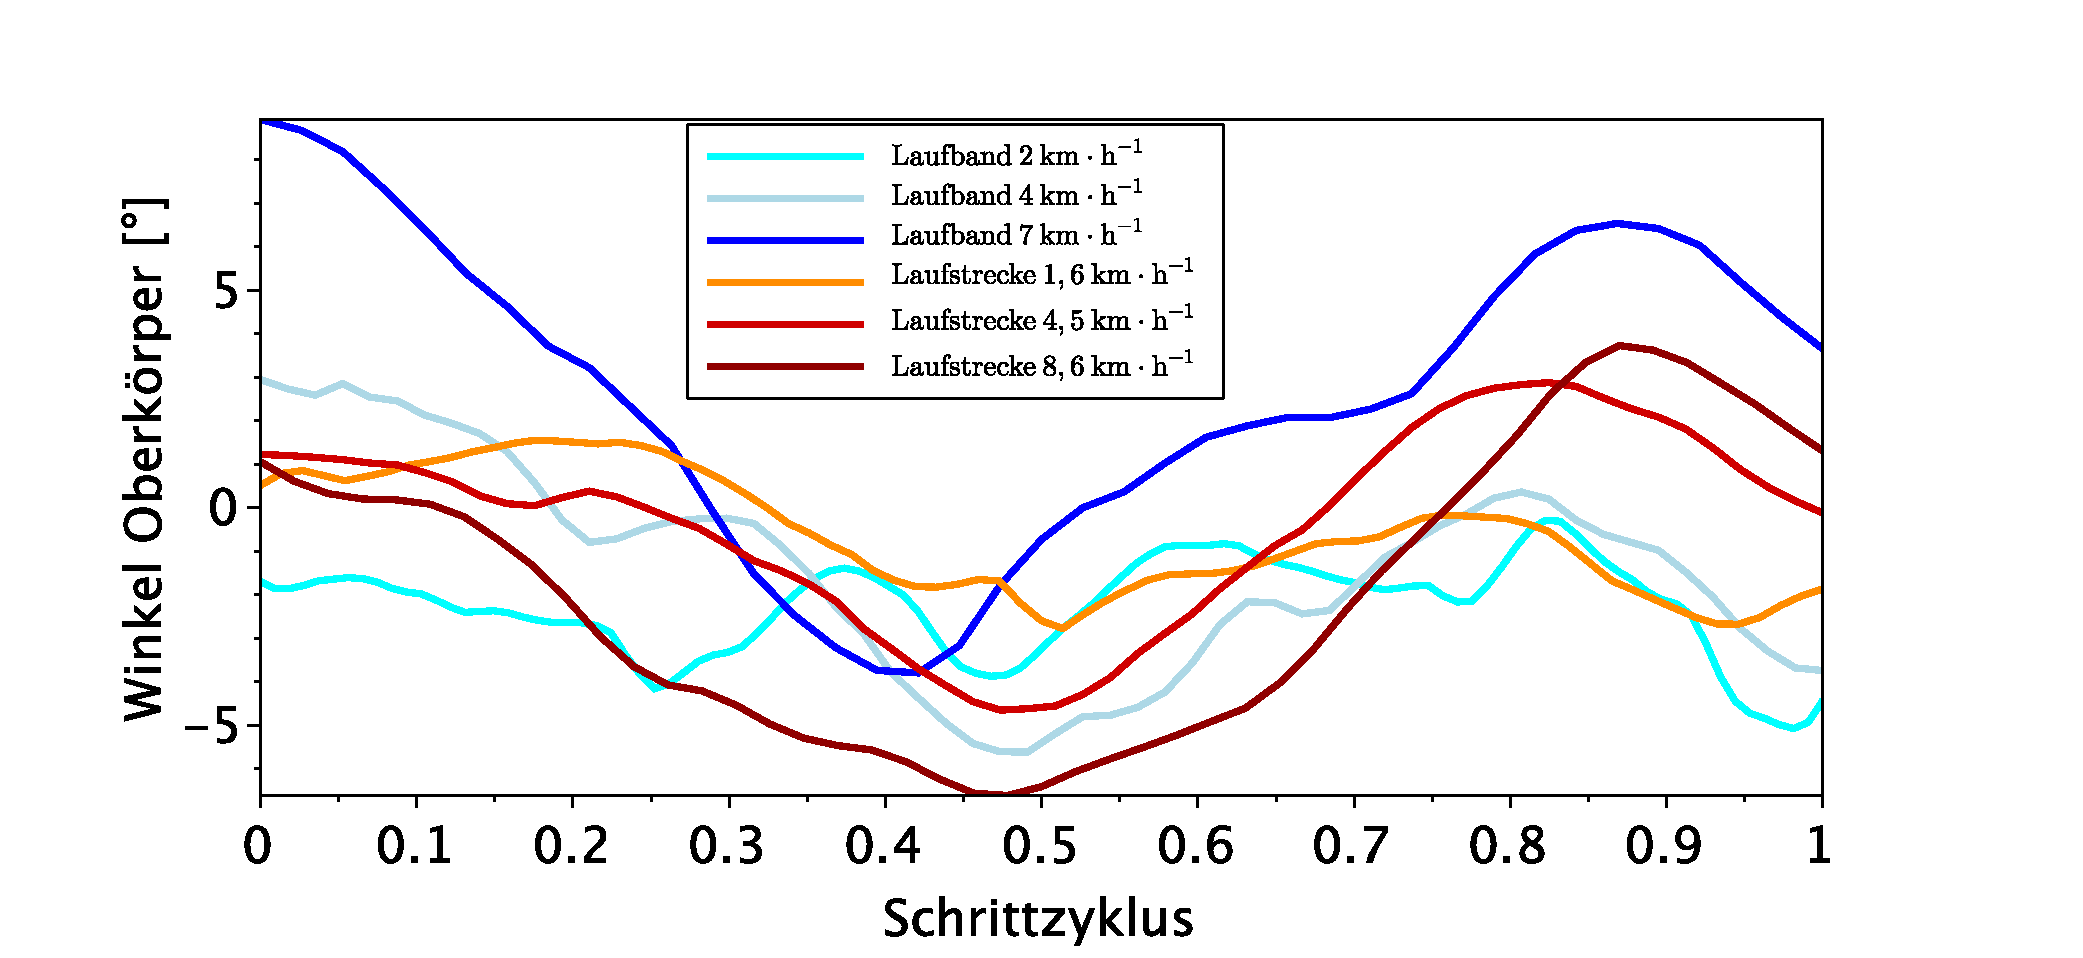
\includegraphics[width=1\linewidth]{bilder/ergebnisse/back_angle.pdf}
	\caption[Bodenreaktionskräfte]{Neigung des Oberkörpers. Negative Werte entsprechen einem Zurücklehnen, positive Werte einem Vorlehnen. Winkelwerte wurden mit einem gleitenden Mittelwert in zwei Durchläufen geglättet.}
	\label{fig:vergleich_oberkörper}
\end{figure}
